\documentclass[11pt,a4paper]{article}
\usepackage[T1]{fontenc}
\usepackage[spanish]{babel}
\usepackage[margin=2.5cm]{geometry}
\usepackage{graphicx}
\usepackage{tabularx}
\usepackage[backend=biber,style=ieee]{biblatex}
\usepackage{xurl}
\usepackage[hidelinks]{hyperref}
\addbibresource{referencias.bib}

\newcommand{\pendiente}[1]{\par\smallskip\noindent\textit{Pendiente: #1}\par}

\begin{document}

\begin{titlepage}
  \centering
  {\Large Universidad Técnica Estatal de Quevedo\par}
  \vspace{0.7em}
  Facultad: por confirmar\par
  Carrera: Ingeniería de Software\par
  Aplicaciones Distribuidas\par
  \vfill
  {\LARGE\bfseries Entrega y recuperación de mensajes en Discord\par}
  \vspace{0.5em}
  {\large Comparación con Zulip\par}
  \vspace{1.5em}
  TA-IND-01\par
  Borrador de trabajo\par
  \vfill
  Byron Daniel Loor Mendoza\par
  Paralelo: por confirmar\par
  Fecha de entrega: por confirmar\par
  \vspace{1em}
  \href{https://github.com/Yukisan-uwo/TA-IND-01-Informe-Academico-Individual-Analisis-Critico-de-Sistemas-Distribuidos-Grupo}{Repositorio del informe}
\end{titlepage}

\begin{abstract}
Este informe analiza la entrega y el almacenamiento de mensajes de texto
en Discord y los compara con Zulip, una plataforma de chat para equipos.
La comparación se apoya en la documentación técnica de ambos sistemas y
considera la arquitectura, los protocolos, las transparencias, la
consistencia, la latencia y la recuperación ante fallos. Se realizó una
prueba con un navegador en una laptop y la aplicación de Discord en un
teléfono conectado por datos móviles. Durante el corte de la laptop se
enviaron tres mensajes desde el teléfono. Al reconectar, los tres
aparecieron en Chrome en el mismo orden, sin duplicados visibles ni
recarga manual. La prueba permitió observar la recuperación del estado
visible del cliente. La documentación de almacenamiento y el incidente
de autenticación de Discord permiten examinar, por separado, cómo la
carga, la replicación y los fallos afectan al servicio. En Zulip, el
análisis distingue el historial persistente en PostgreSQL de la cola
que entrega eventos. El resultado de la prueba tiene alcance local y
el análisis de garantías internas depende de la operación y de la
configuración documentadas.
\end{abstract}

\section{Introducción}
La pregunta del informe es qué compromisos entre latencia, consistencia y
recuperación ante fallos se observan en la entrega y el almacenamiento de
mensajes de texto en Discord, y cómo se comparan con los de Zulip.
Los canales permiten que comunidades conversen en tiempo real y que
quienes se conectan después consulten lo publicado. Esto requiere
resolver dos problemas relacionados: conservar el historial y avisar a
los clientes cuando hay actividad nueva. Discord Engineering describe
una migración de un historial de billones de mensajes que pasó de 177
nodos de Cassandra a 72 de ScyllaDB, según el reporte de 2023
\cite{ingram2023messages}. Zulip también ofrece chat por canales y
organiza conversaciones por temas para equipos que trabajan de forma
sincrónica o en horarios distintos \cite{abbott2026zulip}.
\pendiente{Añadir la razón personal para elegir Discord.}

\section{Arquitectura}
La API HTTP permite solicitar el historial y crear mensajes. La
arquitectura publicada por Discord ubica servicios de datos entre la API
y los clústeres de ScyllaDB. Los servicios exponen operaciones gRPC y
pueden reunir solicitudes simultáneas de una misma fila en una sola
consulta. Discord también describe un enrutamiento por identificador de
canal que ayuda a reunir solicitudes relacionadas en una instancia
\cite{ingram2023messages}.

El Gateway entrega eventos por WebSocket. La ruta de entrega de eventos
y la consulta del historial son operaciones distintas: una mantiene
actualizado al cliente conectado y la otra obtiene mensajes que ya se
guardaron. La API pública describe la reanudación de sesiones para
aplicaciones, que usan un identificador de sesión y un número de
secuencia \cite{discordGateway}.
\pendiente{Incorporar el diagrama digital elaborado por Byron y explicar cómo evolucionó desde su bosquejo.}

\section{Conceptos de sistemas distribuidos}
\subsection{Transparencias}
\begin{description}
  \item[Acceso.] Desde el cliente se consulta un canal a través de la
  API. La interfaz oculta las operaciones del motor de almacenamiento.
  \item[Ubicación.] El usuario trabaja con un identificador de canal. La
  API y el enrutamiento interno resuelven dónde atender la solicitud.
  \item[Migración.] Durante el cambio de Cassandra a ScyllaDB, Discord
  escribió datos nuevos en ambos motores y contrastó una muestra de
  lecturas antes del cambio de base principal \cite{ingram2023messages}.
  \item[Reubicación.] La documentación consultada permite analizar el
  traslado de datos durante la migración. El efecto de mover en caliente
  un servicio mientras procesa una solicitud queda sin verificar.
  \item[Replicación.] El usuario ve un historial. La selección y
  coordinación de copias corresponde a la infraestructura, como se
  documenta para el clúster de autenticación \cite{smith2023authOutage}.
  \item[Concurrencia.] Solicitudes simultáneas de la misma fila pueden
  compartir una consulta al almacenamiento \cite{ingram2023messages}.
  El orden observado en la prueba corresponde a un solo emisor.
  \item[Fallos.] La interfaz puede mostrar la pérdida de conexión.
  En la prueba, la actualización del historial visible se recuperó
  automáticamente después de reconectar la laptop.
\end{description}

\subsection{CAP y PACELC}
Para CAP, interesa qué puede responder una operación si parte de las
réplicas queda incomunicada. Discord describe lecturas por cuórum en el
clúster de autenticación, con datos repartidos en tres zonas. Si una
partición deja a un lado sin el cuórum requerido, una lectura en ese
lado no puede completar con esa política. Durante el incidente
documentado, el problema observado fue de disponibilidad de
autenticación bajo mantenimiento y degradación de recursos
\cite{smith2023authOutage}. El análisis de sistemas replicados de alta
disponibilidad ayuda a identificar qué propiedades pueden debilitarse
ante fallos \cite{kokocinski2023correctness}.

La parte de PACELC que se aplica en operación normal pregunta cuánto
cuesta coordinar réplicas frente a responder con menor latencia. En un
sistema con lecturas por cuórum, esperar a varias réplicas introduce
una dependencia de sus tiempos de respuesta. Las mediciones publicadas
de configuraciones NoSQL muestran que el efecto de variar la
consistencia depende del motor, la operación y el despliegue
\cite{ferreira2024consistency}. Discord reportó que el percentil 99 de
lectura de historial pasó de 40--125 ms con Cassandra a 15 ms con
ScyllaDB después de su migración y cambios de arquitectura
\cite{ingram2023messages}. Ese dato describe una mejora observada y no
identifica por sí solo la política de consistencia del historial.

\subsection{Modelos de comunicación}
Discord sigue un modelo cliente-servidor. En HTTP, el cliente inicia la
solicitud y recibe una respuesta. El Gateway usa un WebSocket persistente
para entregar eventos asíncronos a aplicaciones conectadas
\cite{discordGateway}. En la ruta interna de almacenamiento, gRPC
permite invocar operaciones remotas del servicio de datos
\cite{ingram2023messages}. La separación de eventos y solicitudes
permite que distintas partes progresen a ritmos diferentes. En
arquitecturas por eventos, esa separación obliga a especificar qué
significa que dos componentes hayan sincronizado su estado
\cite{bacao2026consistency}.

\subsection{Tolerancia a fallos}
El informe de Discord sobre el 6 de noviembre de 2023 describe cómo el
mantenimiento de una zona y un disco degradado en otra redujeron la
capacidad del clúster de autenticación. Los reintentos añadieron carga y la
interrupción afectó la lectura y el envío de mensajes
\cite{smith2023authOutage}.
Durante ese incidente, Discord observó tiempos de espera en las
solicitudes de autenticación. La pérdida temporal de capacidad durante
la actualización redujo el margen disponible ante el disco degradado.
Tras la recuperación, el equipo amplió el clúster y revisó el proceso
de actualización \cite{smith2023authOutage}. La replicación ayuda a
tolerar la pérdida de una zona, pero la capacidad de las restantes
también condiciona el servicio. Los reintentos pueden agravar la
sobrecarga cuando muchas solicitudes fallan a la vez.

\section{Experimento}
\subsection{Piloto asistido}
El 12 de noviembre de 2026, Codex operó dos clientes web en una PC.
Chrome recibió el mensaje de control \texttt{BYRON-PILOTO-M0}. El segundo
mensaje, \texttt{BYRON-PILOTO-M1}, apareció en Chrome mientras DevTools aún
mostraba \texttt{Offline}. El ajuste no aisló al receptor en esta ronda,
por lo que el piloto no permite medir la recuperación tras un corte.

\subsection{Prueba principal}
En la primera ronda, Byron comprobó la recepción de un mensaje de control
en Chrome. Durante el corte envió tres mensajes desde el celular. Una
captura del navegador posterior al envío aún mostraba solo el mensaje de
control de esta ronda. Al reconectar, los tres mensajes aparecieron sin
recarga manual. La captura posterior muestra una entrada de cada mensaje,
en orden M1, M2 y M3. La hora visible corresponde a la captura. El
tiempo de recuperación quedó sin medir.
La laptop usó Chrome y el teléfono permaneció conectado con datos
móviles. Los comandos \texttt{Get-Date}, \texttt{whoami} y
\texttt{Write-Output} registraron la hora, el usuario y las
observaciones manuales. El procedimiento está en
\texttt{resultados/EXPERIMENTO.md}. La transcripción original está en
\path{resultados/sesion-20261112-233908.txt} e incluye una anotación
posterior sobre la reconexión.

\begin{figure}[p]
  \centering
  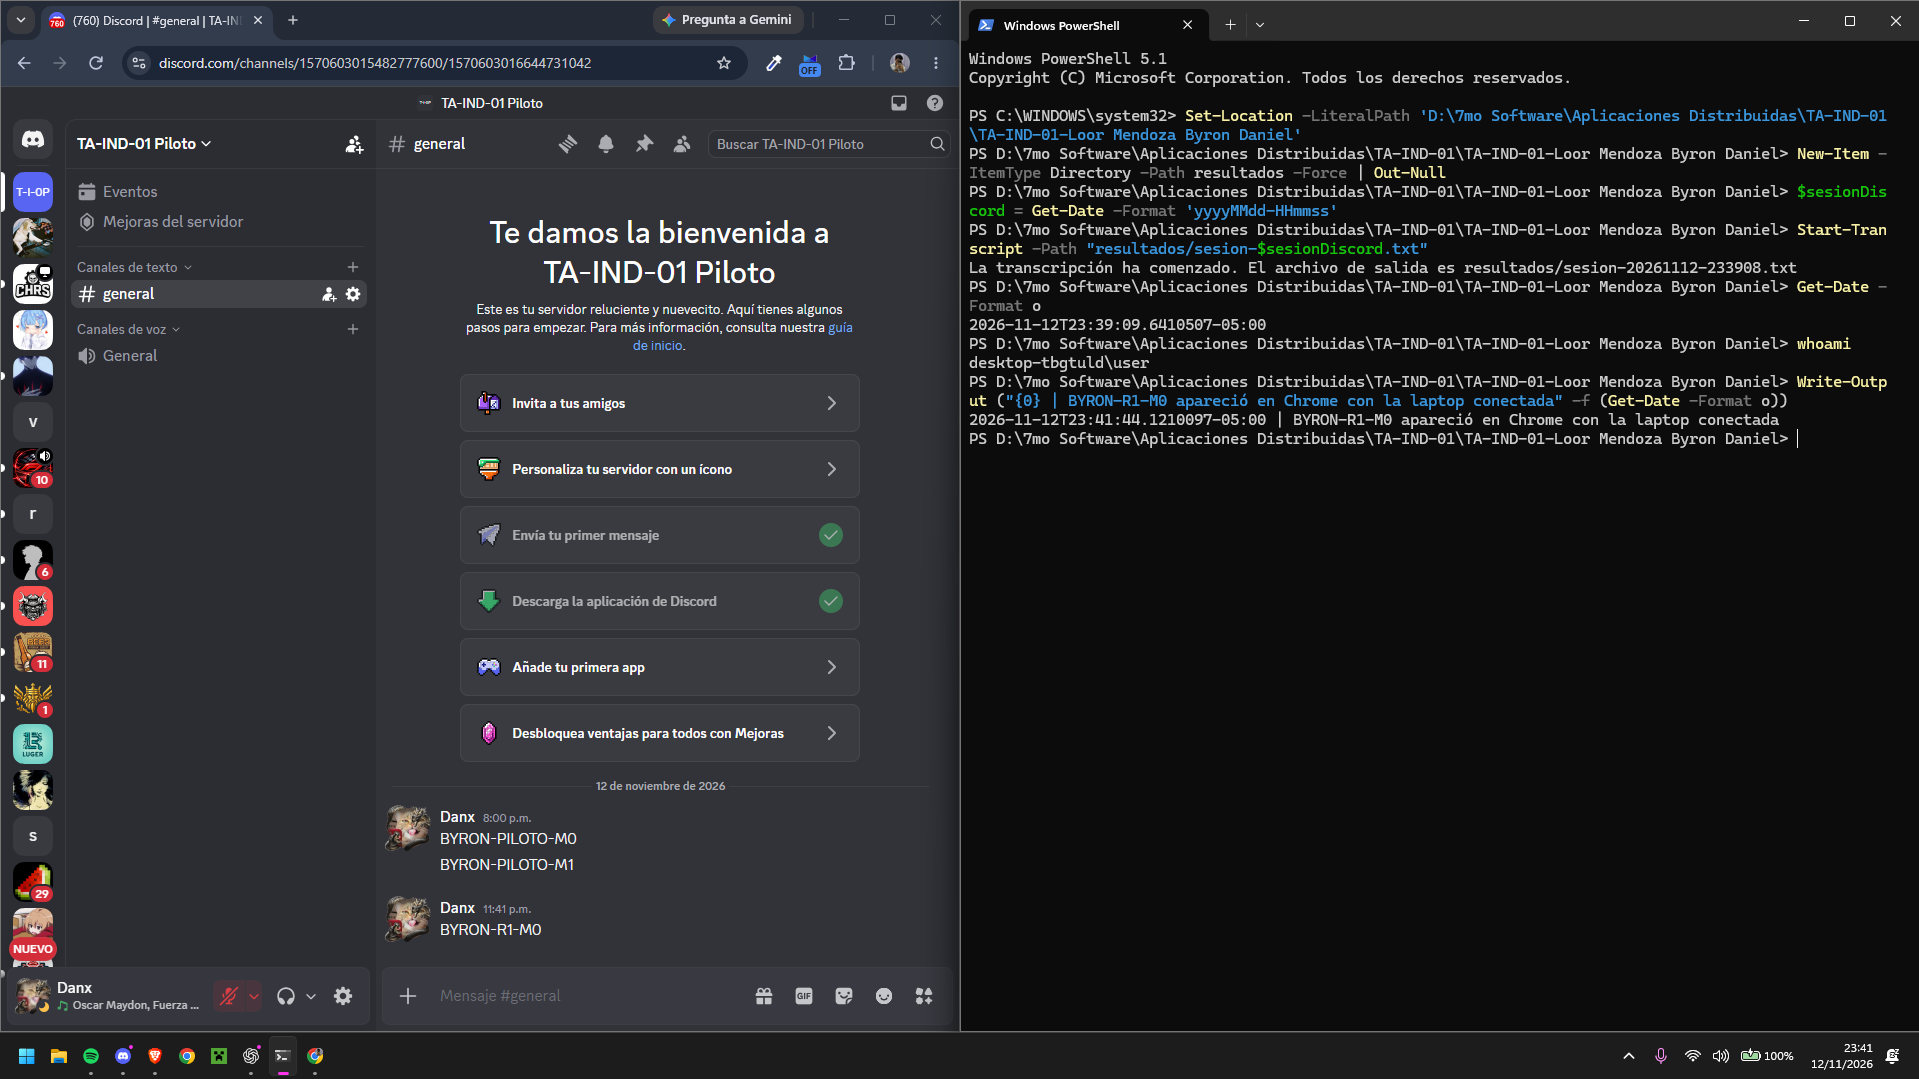
\includegraphics[width=\linewidth]{../resultados/capturas/02-mensaje-recibido.png}
  \caption{Mensaje de control visible en Chrome con la laptop conectada.}
  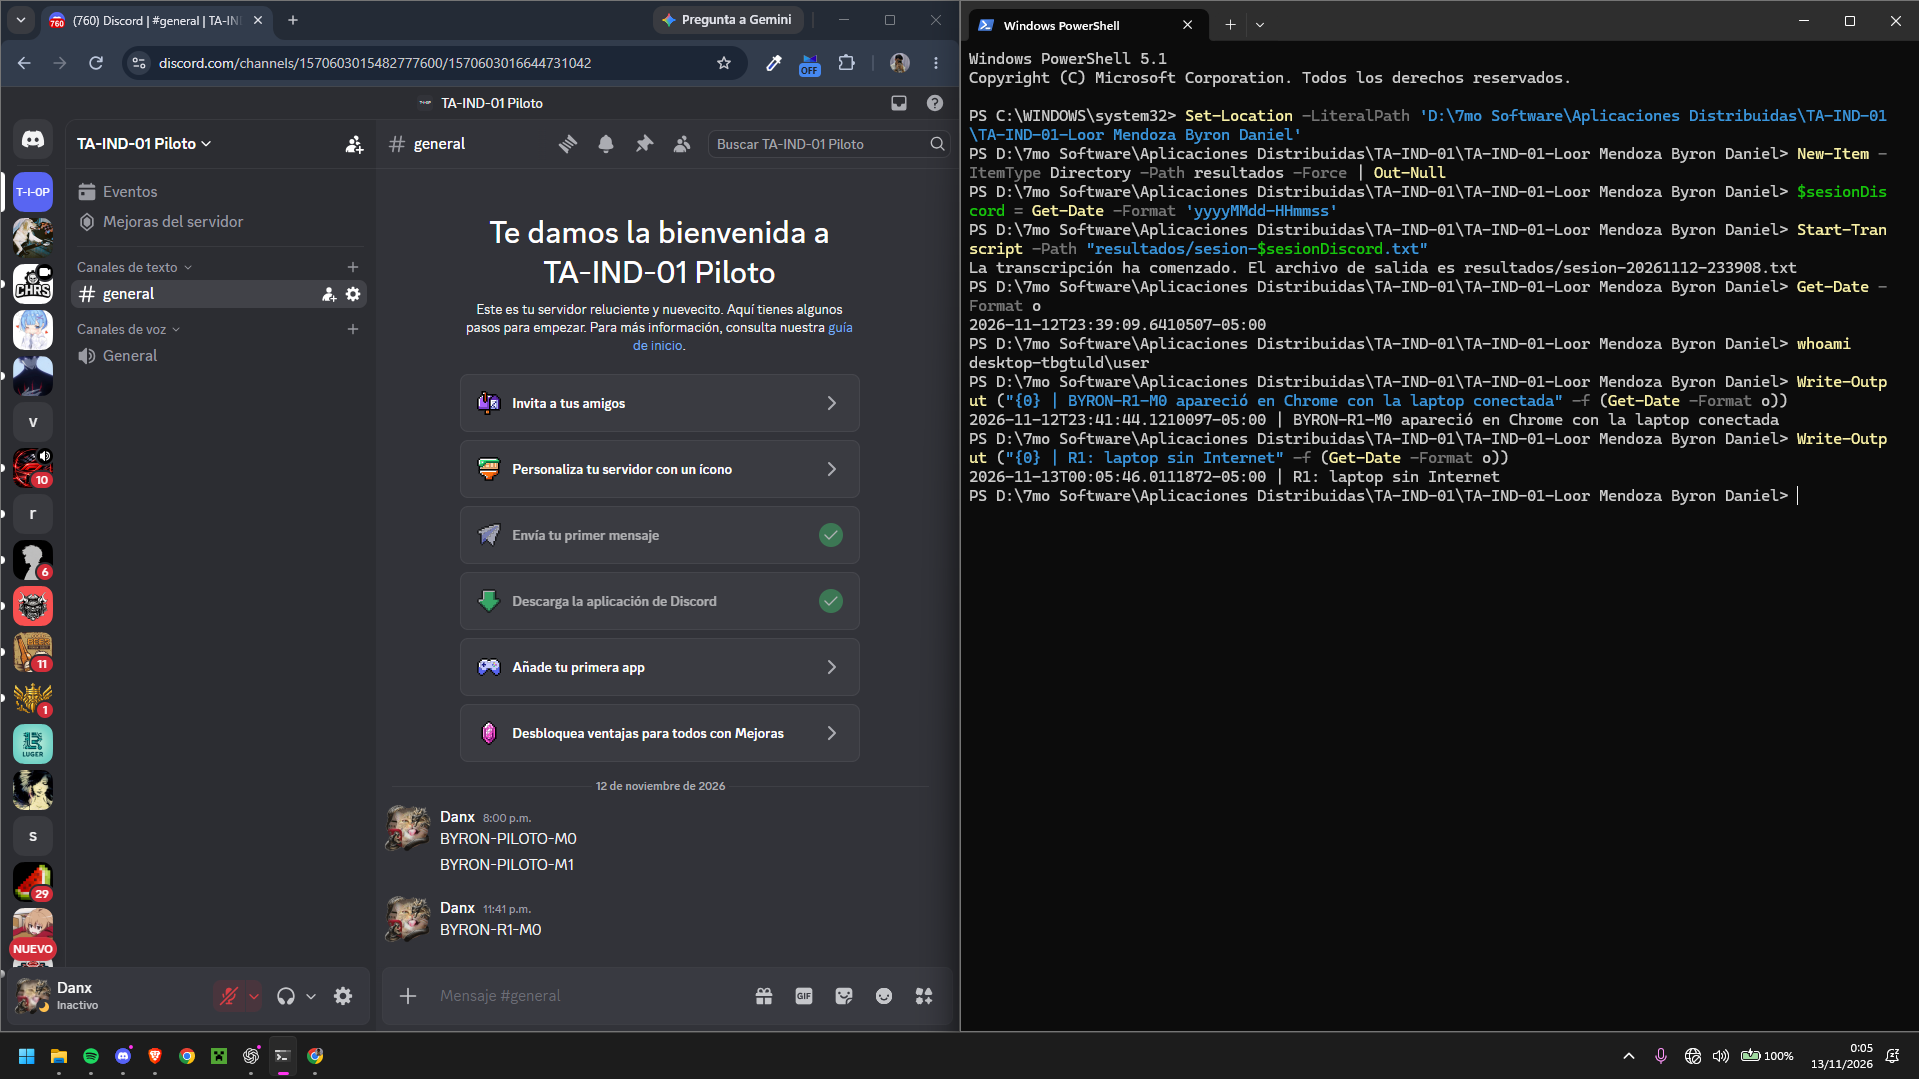
\includegraphics[width=\linewidth]{../resultados/capturas/03a-inicio-del-corte.png}
  \caption{Inicio del corte con el indicador de red de Windows sin Internet.}
\end{figure}

\begin{figure}[p]
  \centering
  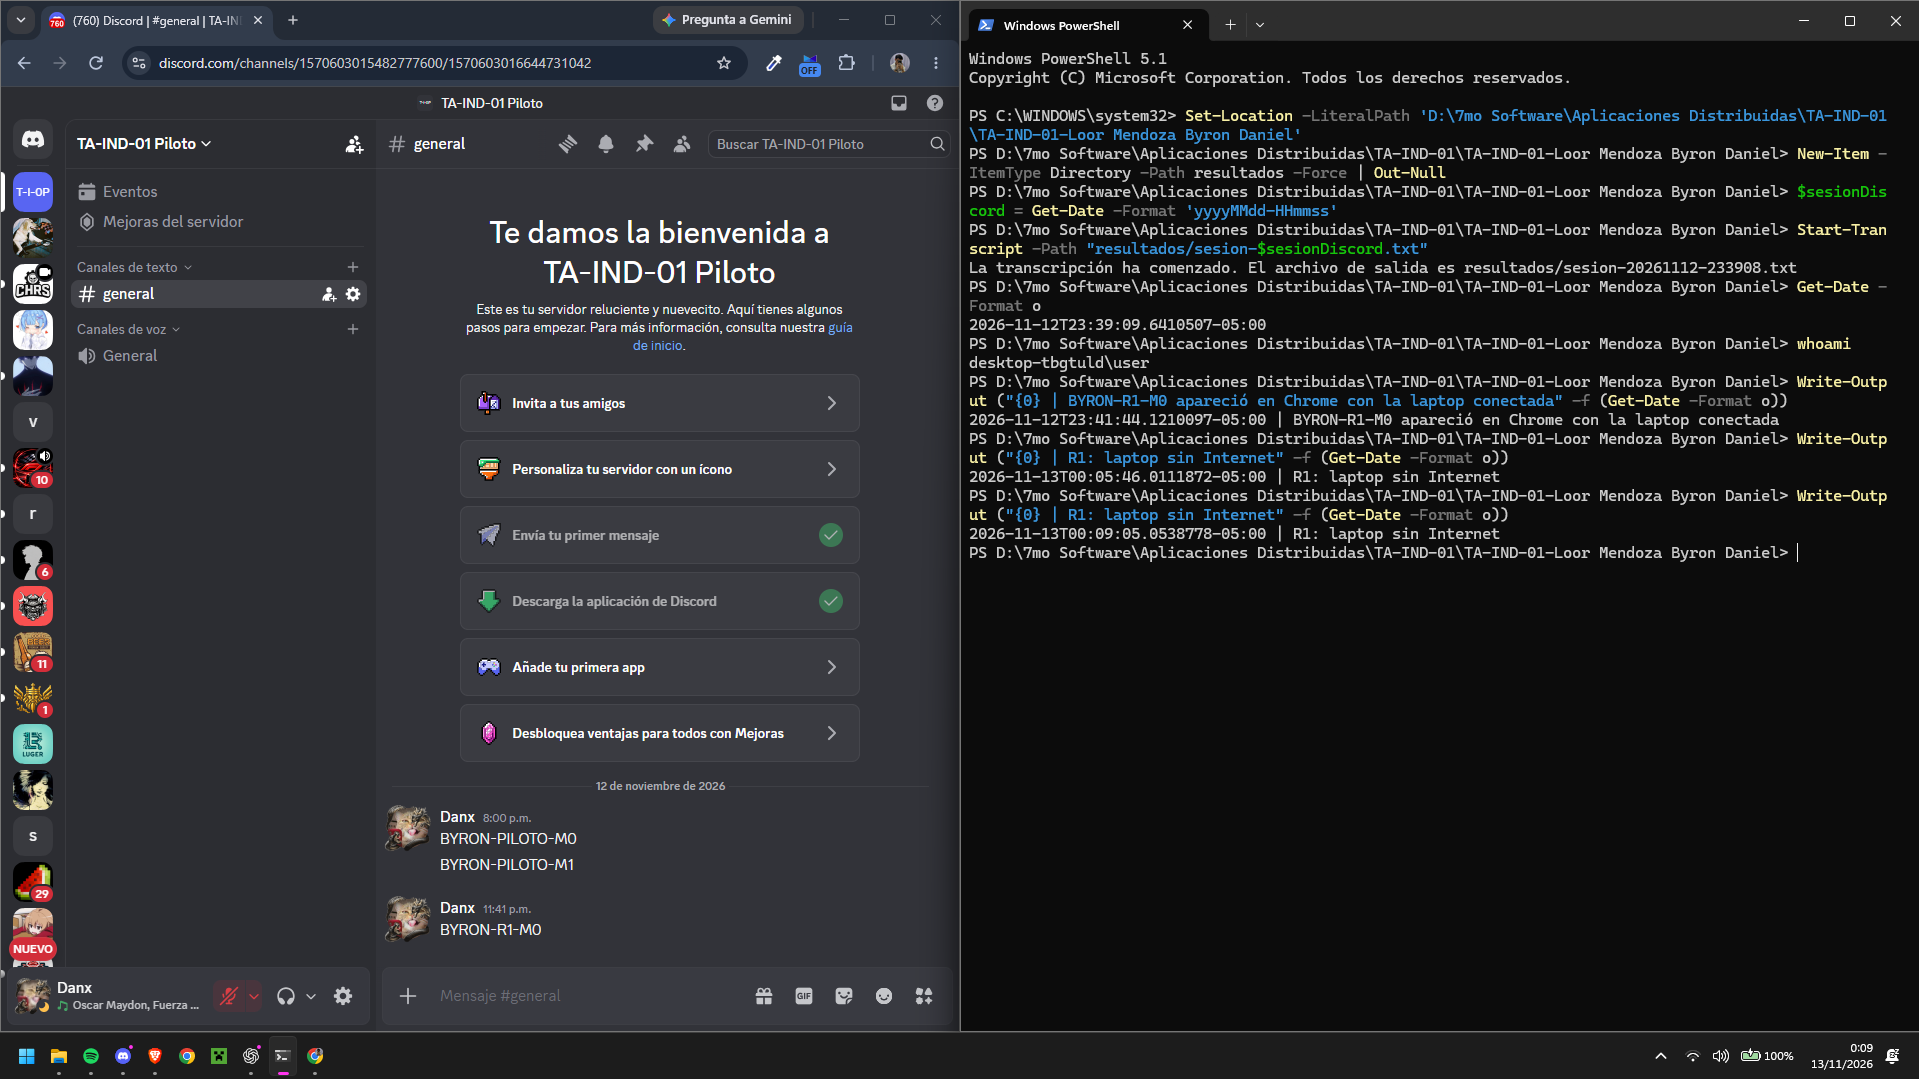
\includegraphics[width=\linewidth]{../resultados/capturas/03b-chrome-despues-del-envio.png}
  \caption{Chrome aún muestra M0 a las 00:09. El registro manual y el icono de Wi-Fi se conservan como aparecen en la captura.}
  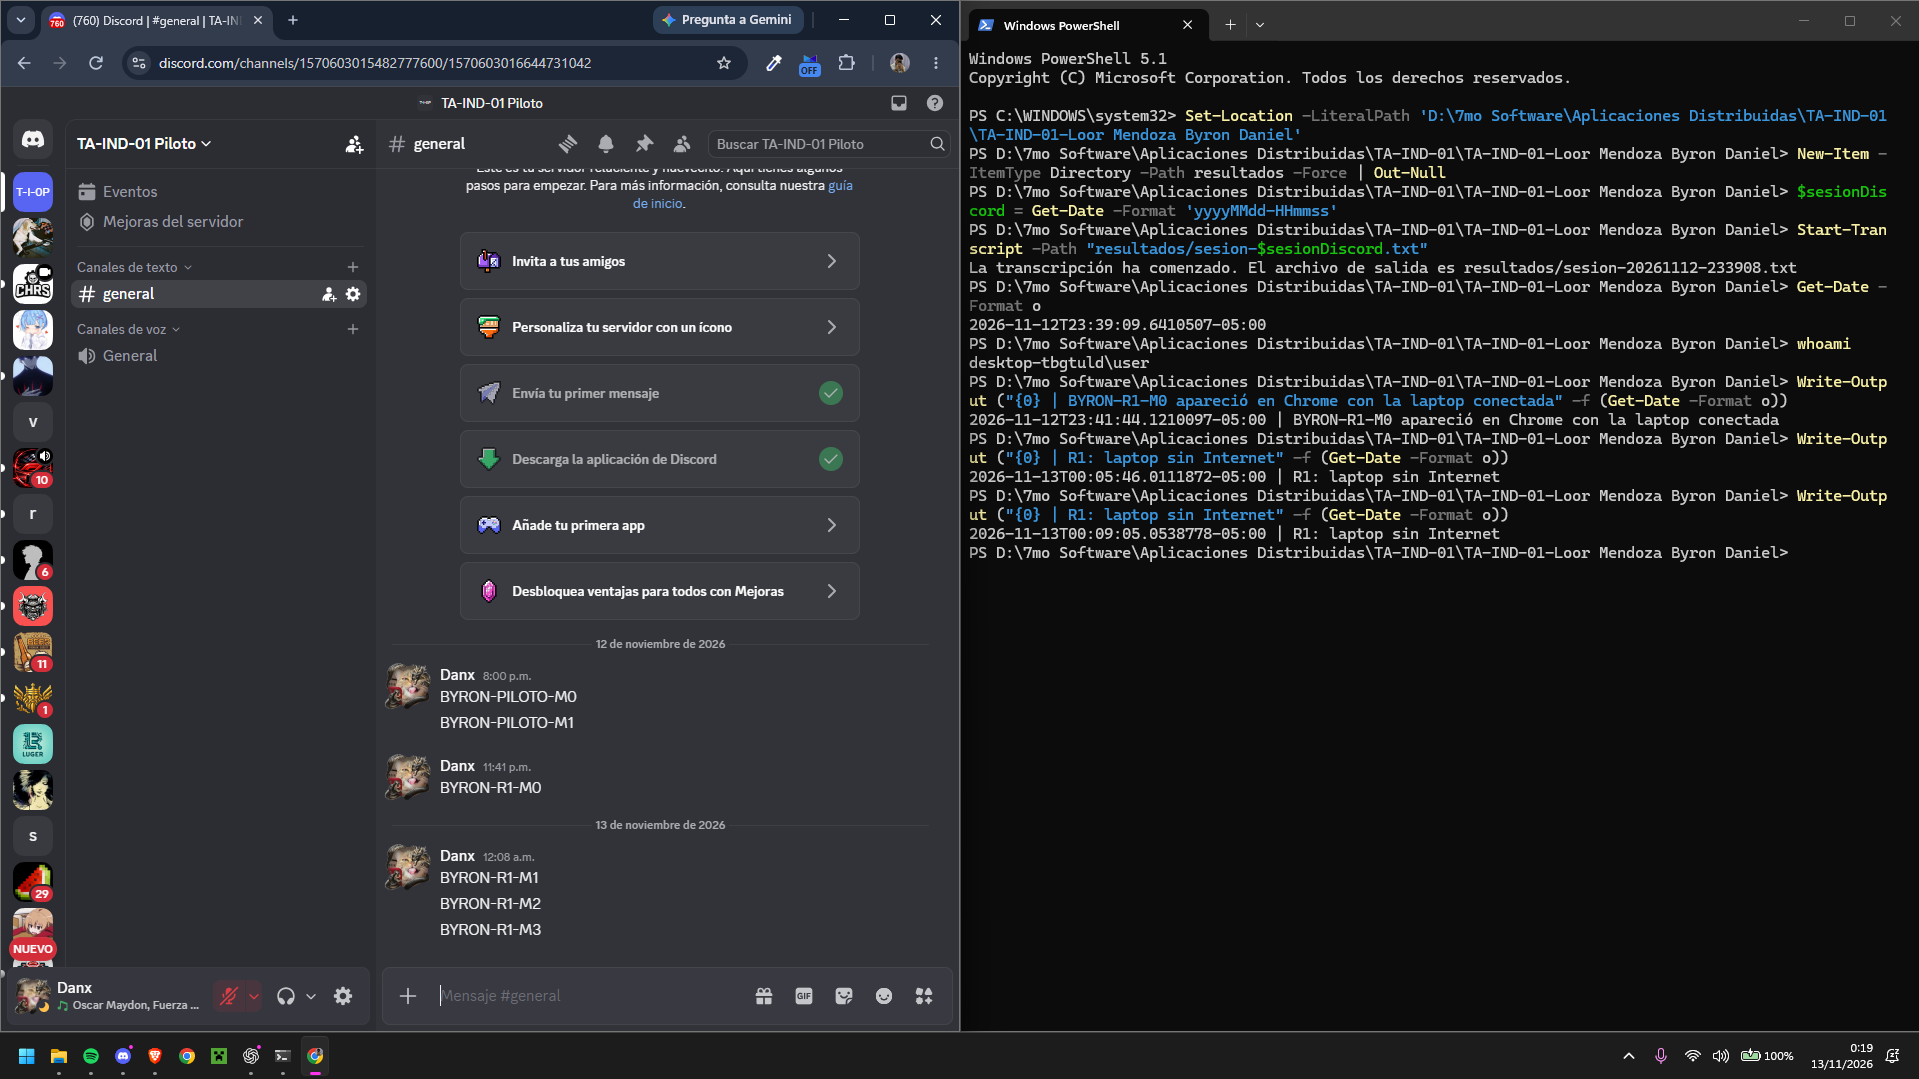
\includegraphics[width=\linewidth]{../resultados/capturas/04-reconexion.png}
  \caption{Estado capturado a las 00:19 con los tres mensajes visibles después de reconectar.}
\end{figure}
\clearpage

El resultado describe la recuperación del estado visible del cliente.
La prueba interrumpió el acceso a la red de una laptop y mantuvo el
teléfono conectado. Las réplicas del servicio quedaron fuera del
control experimental. Por eso, la observación no permite clasificar
Discord según CAP ni identificar si el cliente reanudó una sesión del
Gateway o consultó el historial.

\section{Ejemplos del entorno}
\paragraph{Discord y el aviso de reconexión.}
Cuando se corta mi conexión, he visto el aviso «Reconectando» en la zona
del micrófono de Discord. Cuando vuelve Internet, la aplicación cambia
de estado. Esto ilustra una transparencia a fallos parcial: el cliente
puede gestionar la reconexión y, al mismo tiempo, hacer visible la
interrupción al usuario.

\paragraph{Zulip y el historial por temas.}
En la demo de Zulip, Byron envió \texttt{ZULIP-M1} al tema
\textit{Prueba TA-IND-01} del canal \texttt{\#general}. Con apoyo de
Codex se abrió el tema \textit{saludos} y luego se volvió a
\textit{Prueba TA-IND-01}, donde el mensaje seguía visible. El ejemplo
ilustra la transparencia de acceso: el usuario consulta el historial
por canal y tema desde la interfaz, que se encarga de obtener los datos.
La figura~\ref{fig:zulip-tema} muestra el resultado de la comprobación.

\section{Comparación con Zulip}
La comparación considera Discord como servicio administrado y Zulip
como una instalación con servidor de aplicación y PostgreSQL
separados, según la configuración documentada
\cite{ingram2023messages,zulipArchitecture,zulipPostgresql}.

\begin{center}
\small
\begin{tabularx}{\linewidth}{|p{0.22\linewidth}|X|X|}
\hline
\textbf{Criterio} & \textbf{Discord} & \textbf{Zulip} \\
\hline
Arquitectura & API, servicios de datos y ScyllaDB para el historial. &
Django atiende solicitudes y Tornado entrega eventos. \\
\hline
Comunicación & API HTTP y eventos del Gateway por WebSocket. &
Solicitudes HTTP y espera prolongada mediante \textit{long polling}. \\
\hline
Transparencia de acceso & El cliente consulta mensajes por canal
mediante la API. & El usuario consulta canales y temas mediante la
aplicación, que accede a la base. \\
\hline
Almacenamiento & Particiones de mensajes en el clúster documentado. &
PostgreSQL guarda el mensaje y su relación con los destinatarios. \\
\hline
Consistencia y latencia & Lecturas por cuórum en el caso documentado de
autenticación. & Escritura transaccional en el servidor primario.
La configuración de replicación condiciona la recuperación. \\
\hline
Recuperación & La API Gateway documenta reanudar sesiones para
aplicaciones. & El cliente confirma eventos mediante su último ID.
Si la cola expira, obtiene el estado inicial de nuevo. \\
\hline
\end{tabularx}
\end{center}

Fuentes de la comparación
\cite{ingram2023messages,discordGateway,smith2023authOutage,zulipArchitecture,zulipSendingMessages,zulipPostgresql,zulipEvents}.
Zulip conserva los mensajes en PostgreSQL y usa una cola por cliente
para entregar las novedades. El último identificador recibido permite
solicitar eventos pendientes mientras la cola existe. Si se configura
una réplica de respaldo de PostgreSQL, la recuperación frente a una
caída del primario implica promoverla antes de aceptar escrituras
\cite{zulipEvents,zulipPostgresql}. Son dos recuperaciones distintas:
la del cliente que perdió sus eventos y la del almacenamiento que
debe volver a servir escrituras.

La demo permitió observar la organización del historial por temas en
Zulip. La prueba de Discord observó la recuperación del historial
visible tras un corte de conexión. La comparación de los mecanismos
internos se apoya en la documentación técnica de cada plataforma.

\begin{figure}[htbp]
  \centering
  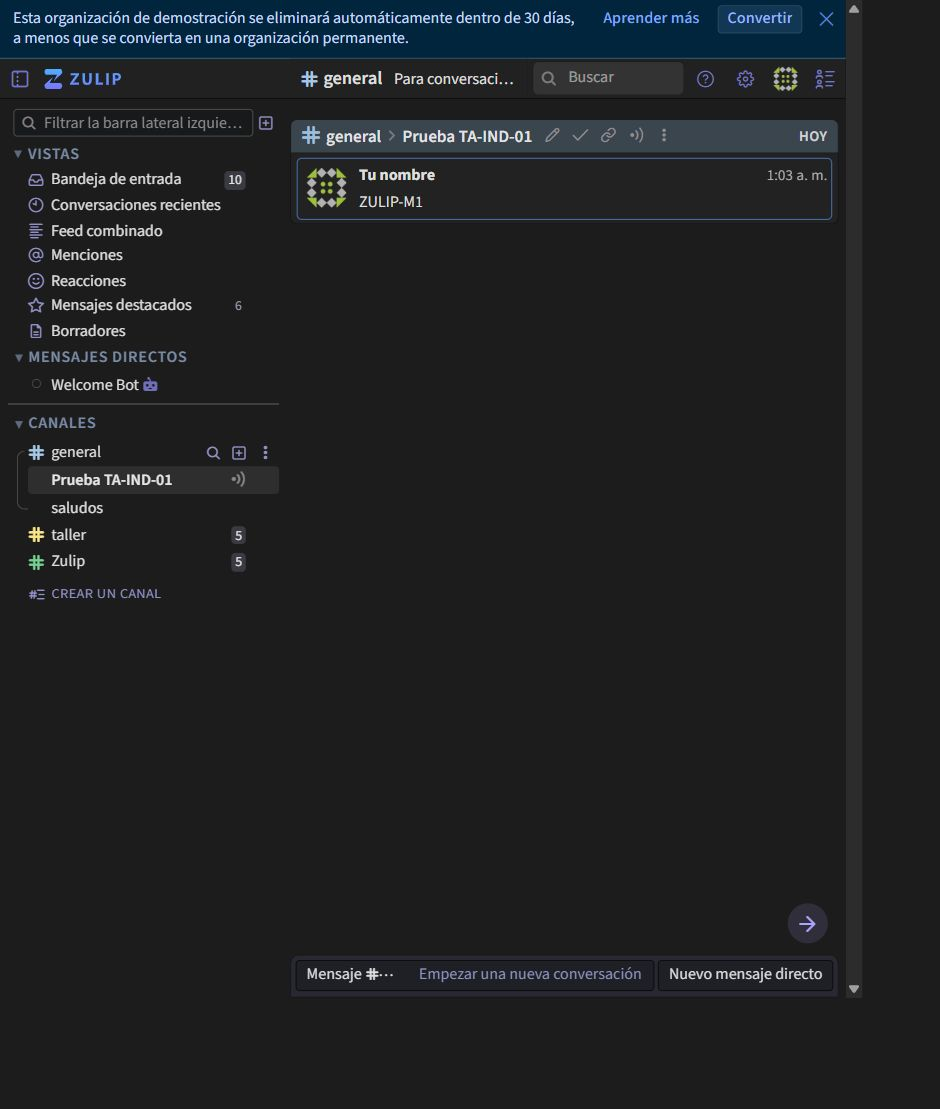
\includegraphics[width=0.56\linewidth,height=0.37\textheight,keepaspectratio]{../resultados/capturas/zulip-tema-prueba.jpg}
  \caption{Mensaje enviado por Byron en el tema de prueba de Zulip. Codex capturó la vista al volver a abrir el tema.}
  \label{fig:zulip-tema}
\end{figure}

\section{Postura crítica}
El diseño de Discord reduce la presión sobre el almacenamiento cuando
muchos usuarios consultan los mismos mensajes. Reunir esas consultas
protege a la base frente a ráfagas, aunque las particiones calientes
siguen siendo un problema que el equipo debe vigilar
\cite{ingram2023messages}. Zulip puede ser preferible si el equipo
necesita administrar el alojamiento y decidir cómo operar su
PostgreSQL. Ese control añade trabajo de respaldo, supervisión y
recuperación al equipo que lo aloja
\cite{abbott2026zulip,zulipPostgresql}.

En ambos casos conviene distinguir entre poder ver un mensaje tras
reconectar y exigir una garantía para todas las operaciones ante un
fallo. Una decisión que dependa de esa garantía requiere precisar la
operación, la configuración de almacenamiento y las condiciones de
fallo que debe soportar.

\section{Conclusiones}
En el ensayo de Discord, Chrome volvió a mostrar los tres mensajes
enviados mientras la laptop estuvo desconectada, en el orden observado
en el teléfono y sin recarga manual. Esto respalda la recuperación del
cliente en la condición ensayada. La comparación explica por qué la
entrega de eventos y la persistencia se evalúan por separado: los
eventos mantienen actualizado al cliente y el historial proporciona una
fuente que se puede consultar tras un corte.

\section*{Declaración de uso de inteligencia artificial}
Se utilizó Codex (modelo GPT-6.1 Sol) para organizar y redactar partes
del borrador, orientar la revisión de fuentes, asistir en el piloto y
ordenar las capturas originales de la prueba que realizó el estudiante.
En Zulip, Codex preparó el borrador del mensaje, verificó que siguiera
visible al volver al tema y tomó la captura. Byron realizó el envío.
\pendiente{Completar la declaración con los usos posteriores y la verificación que realizó el estudiante.}

\clearpage
\printbibliography

\clearpage
\appendix
\section{Bosquejo inicial}
\pendiente{Insertar la foto original del esquema a mano con nombre y fecha visibles.}

\section{Lectura de fuentes}
\pendiente{Insertar tres capturas propias de los artículos con la página visible, la anotación personal y la cita correspondiente.}

\end{document}
